
\documentclass{article}
\usepackage[spanish]{babel}
\usepackage[utf8]{inputenc}
\usepackage{amssymb, amsmath, amsbsy, wasysym}
\usepackage{multirow}
\usepackage{graphicx}
\usepackage{hyperref}
\title{Práctica 4\\Redes de computadoras}
\author{Emmanuel Peto Gutiérrez}
\begin{document}
\maketitle

\section{Pasos para realizar la práctica}

Se registró el dominio \textit{emmanuelpeto.gq} en la página https://www.freenom.com. Para ello se colocó el nombre \textit{emmanuelpeto} en el inicio de la página y se le dio click al botón azul que dice \textit{Comprobar disponibilidad}. En la siguiente página se eligió la extensión \textit{gq} y se dio finalizar compra. El tiempo por el que se eligió el dominio fueron 12 meses (que todavía es gratis). Finalmente se eligió iniciar sesión con Google, con la cuenta de ciencias. Se envió un enlace a mi correo para comprobar la cuenta, llené un formulario y después pude acceder.

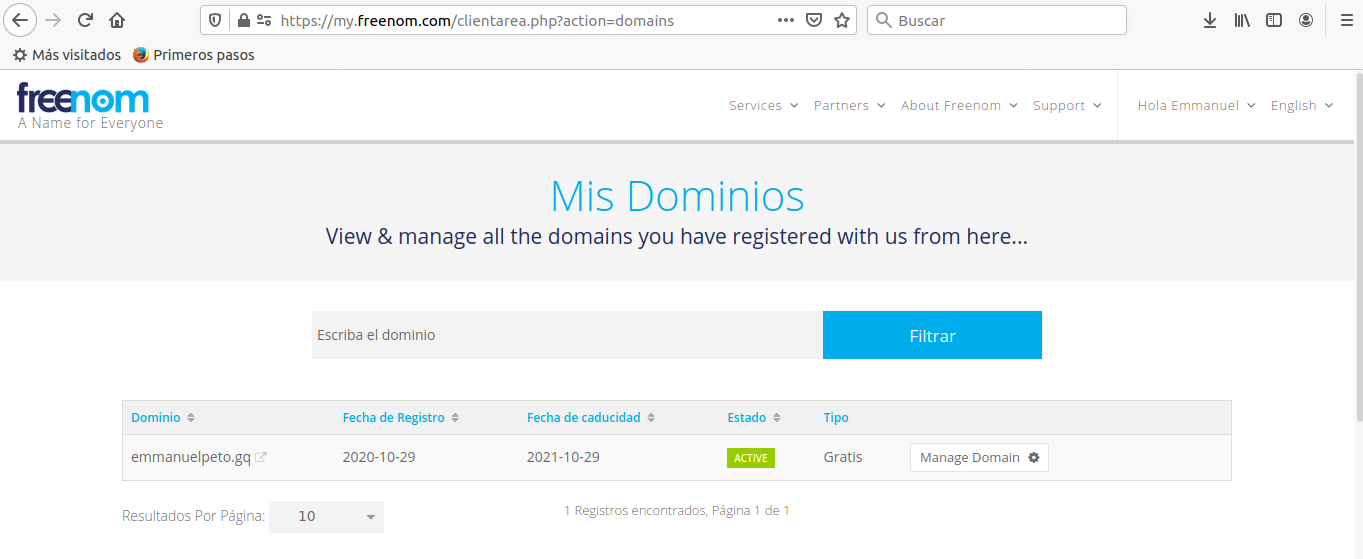
\includegraphics[width=\linewidth]{imagenes/paso1}

En la sección de \textit{Mis dominios} le di click al botón \textit{Gestionar dominio.} Luego le di click en la pestaña \textit{Gestionar DNS Freenom}. En esta página se elige el tipo A (que es para IPv4) y en \textit{Target} se coloca la dirección IP elástica creada en la práctica 3.

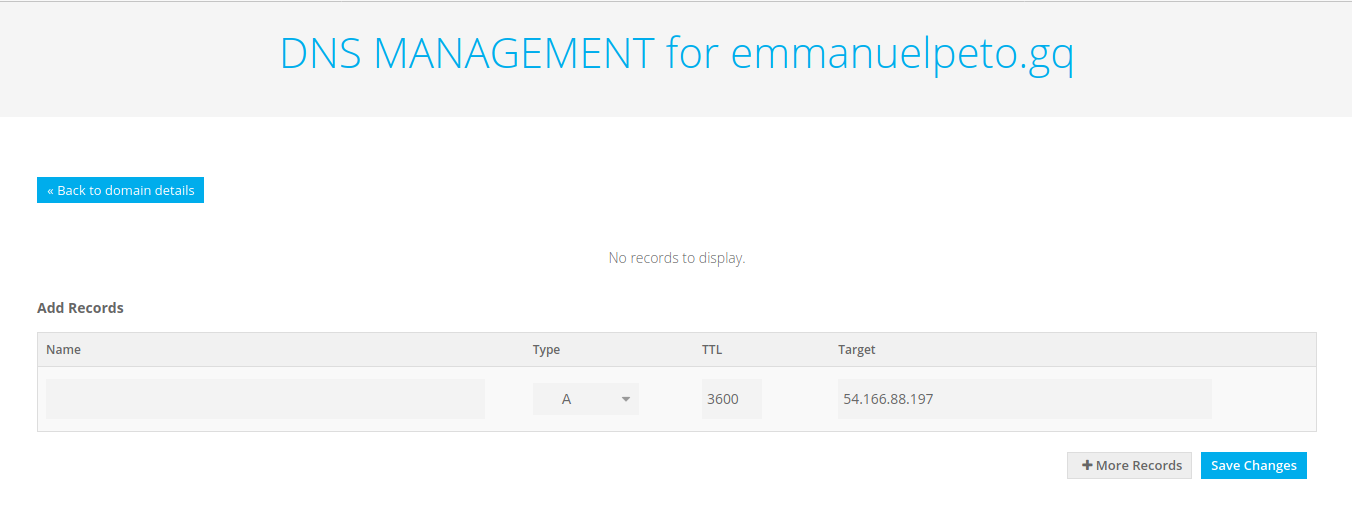
\includegraphics[width=\linewidth]{imagenes/paso2}

Si todo salió bien debería decir \textit{Record added successfully}. Después de un tiempo se debería poder acceder a la página creada en la práctica 3 mediante el nombre de dominio.

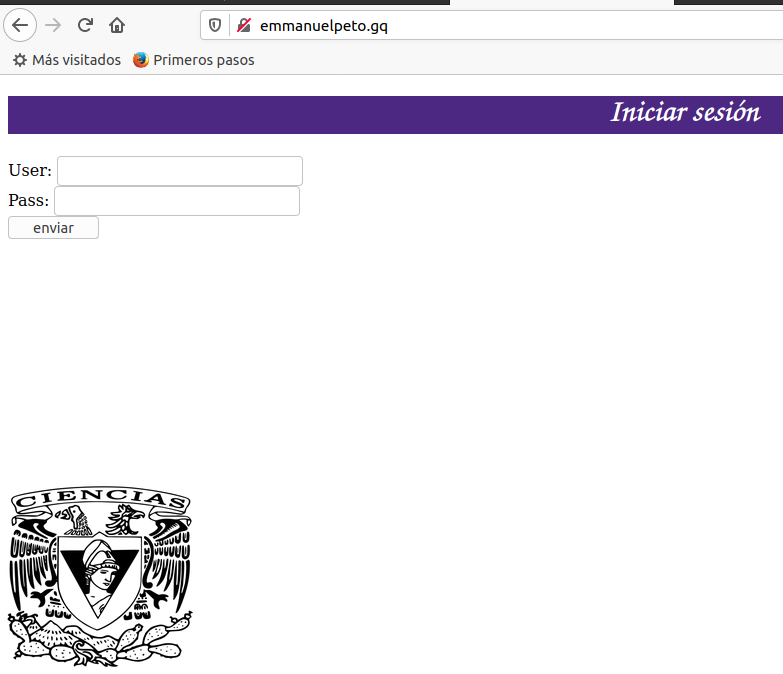
\includegraphics[width=\linewidth]{imagenes/paso3}

Para revisar la propagación del nombre de dominio se usó la página \texttt{dnschecker.org}. Después de 16 horas (más o menos) de haber registrado el nombre de dominio se puede notar que ya se resolvió en todos los servidores DNS que se muestran en la página \texttt{dnschecker}.

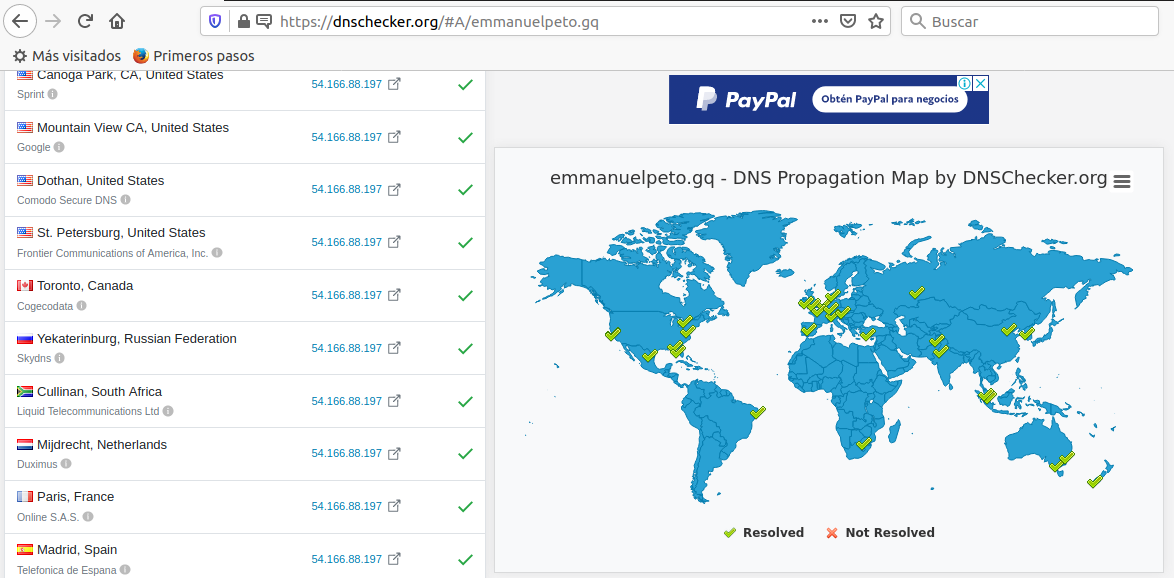
\includegraphics[width=\linewidth]{imagenes/paso4}

El siguiente paso es instalar un certificado de seguridad para el dominio que se acaba de crear. Para ello hay que ver el manual en la página \texttt{letsencrypt.org}. Hay que pinchar el botón \textit{Empezar} de la página principal.

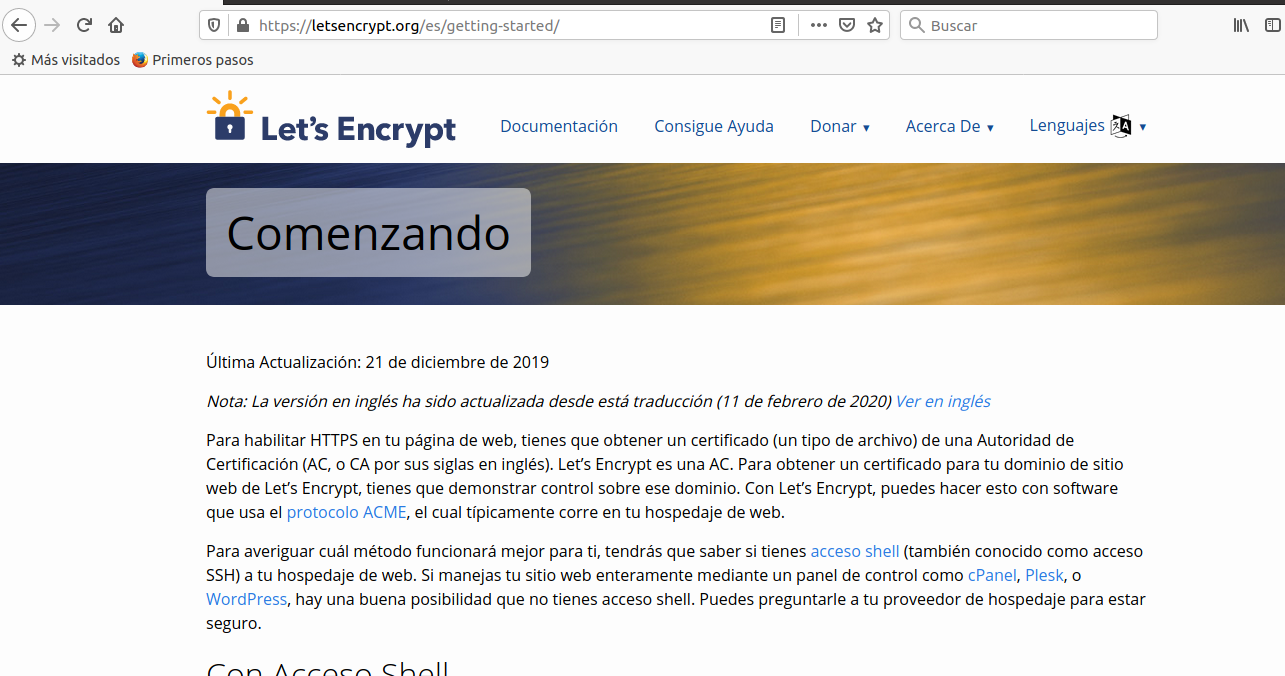
\includegraphics[width=\linewidth]{imagenes/paso5}

Para instalar el certificado hay que leer las instrucciones que dicen \textit{Con acceso Shell}, ya que nosotros nos conectamos al servidor mediante SSH. Hay que hacer click en el enlace que dice \textit{Certbot}.

El enlace nos lleva a la página de Certbot. En esta página hay una sección que dice \textit{My website is running on \_ on \_}, y hay que elegir el servidor Apache y el sistema operativo Ubuntu 20.04, que es el que se instaló en el servidor de AWS.

Una vez elegido el servidor y el sistema operativo se mostrarán las instrucciones para instalar el certificado.

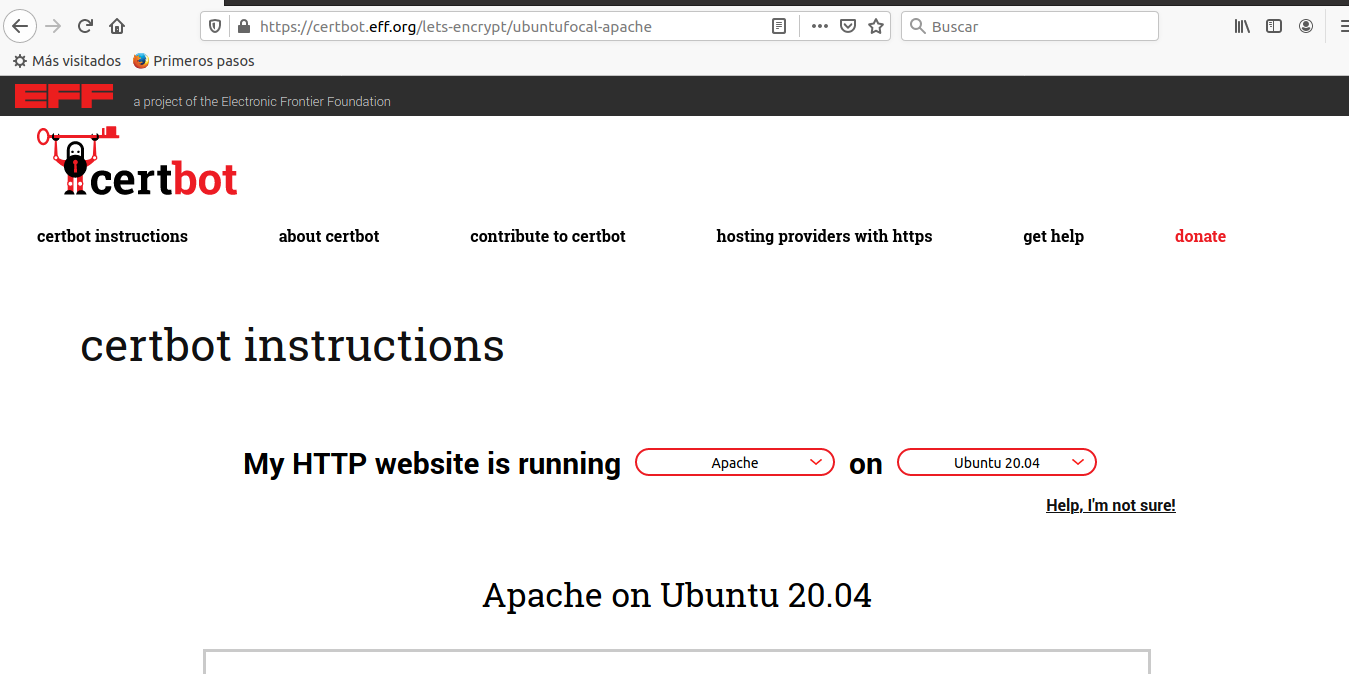
\includegraphics[width=\linewidth]{imagenes/paso6}

\subsection{Certbot}

\begin{itemize}

\item[1.] El primer paso es conectarse con el servidor mediante SSH, como ya se ha mostrado en las prácticas 2 y 3.

\item[2.] Se comprueba que se tenga instalado Snap con los comandos \texttt{sudo snap install core; sudo snap refresh core}.

\item[3.] Desinstalar paquetes Certbot que ya estén instalados en el sistema operativo (si es que lo están). Para esto se usa el comando \texttt{sudo apt-get remove certbot}. En mi caso, no había paquetes certbot instalados previamente.

\item[4.] Después, hay que instalar certbot con el comando \texttt{sudo snap install --classic certbot}.

\item[5.] Para garantizar que se puede ejecutar el comando certbot, ejecutar el siguiente comando: \texttt{sudo ln -s /snap/bin/certbot /usr/bin/certbot}.

\item[6.] Desconectarse del SSH y volverse a conectar pero ahora cambiando la dirección IP por el nombre de dominio. En mi caso:\\ \texttt{ssh -i ``practica2.pem'' ubuntu@emmanuelpeto.gq}.

\item[7.] Ejecutar el siguiente comando para obtener un certificado y que Certbot edite la configuración de Apache automáticamente, encendiendo el acceso a HTTPS en un solo paso: \texttt{sudo certbot --apache}.

\end{itemize}

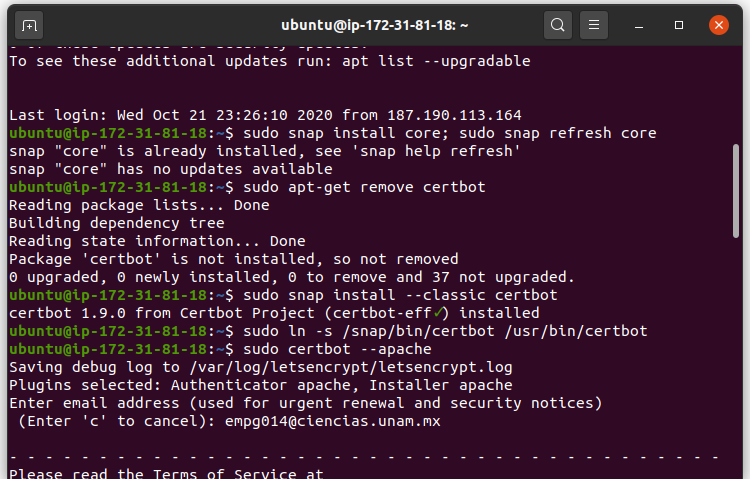
\includegraphics[width=\linewidth]{imagenes/paso7}

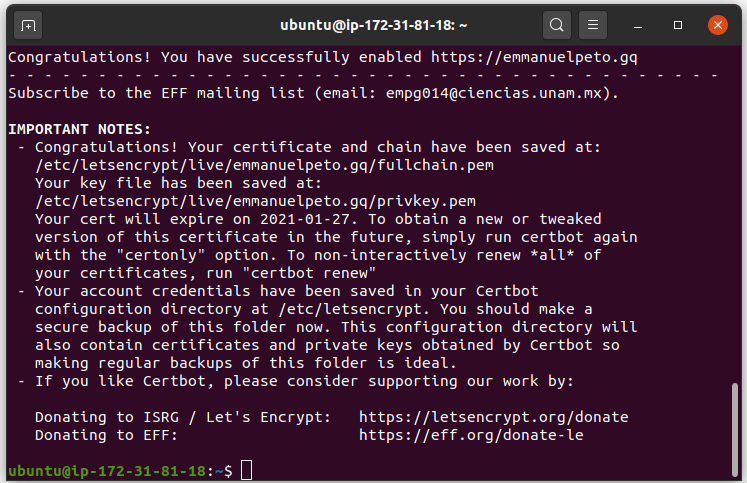
\includegraphics[width=\linewidth]{imagenes/paso8}

Se puede comprobar la renovación automática de los certificados ejecutando el comando: \texttt{sudo certbot renew --dry-run}.

\textbf{Nota:} para poder conectarse mediante HTTPS hay que habilitarlo en el Security Group de AWS. Para esto hay que ir a EC2, buscar en el menú de la izquierda \texttt{Redes y seguridad/Security Groups}, dar click en el grupo de seguridad que se esté usando, dar click en Editar reglas, Agregar regla, elegir HTTPS y guardar.

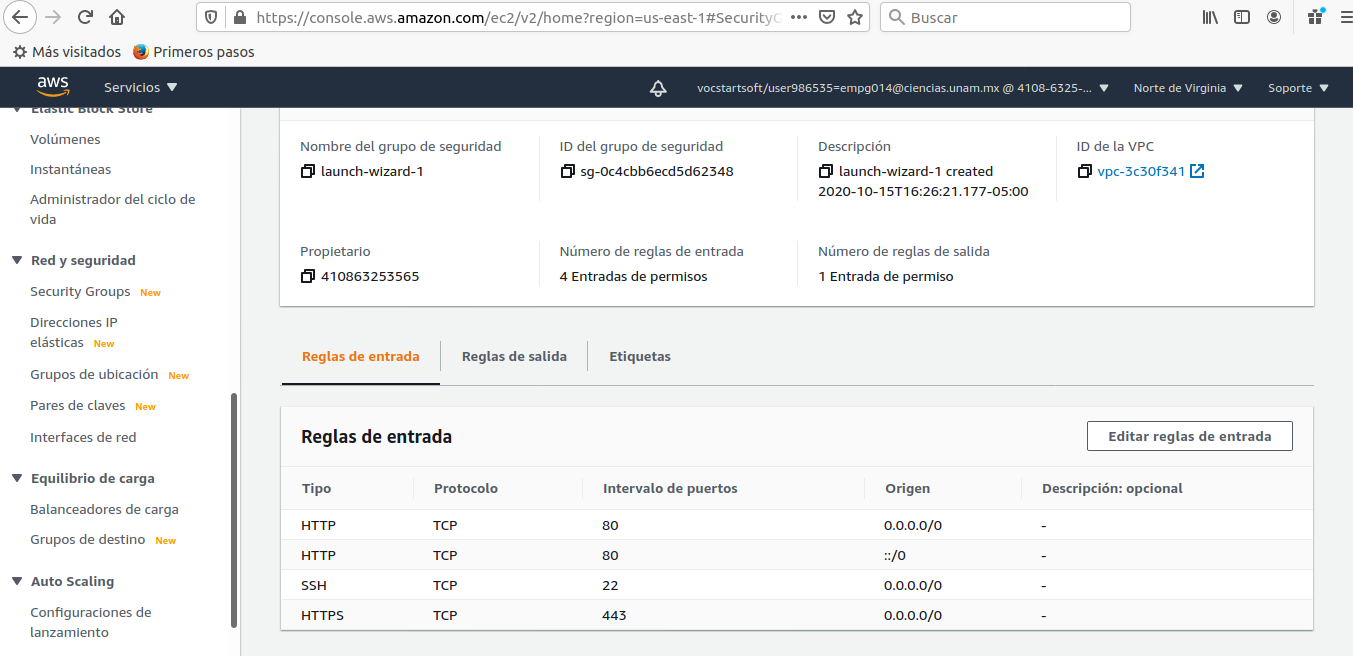
\includegraphics[width=\linewidth]{imagenes/paso9}

Y ahora sí, ya se puede entrar a la página mediante https.

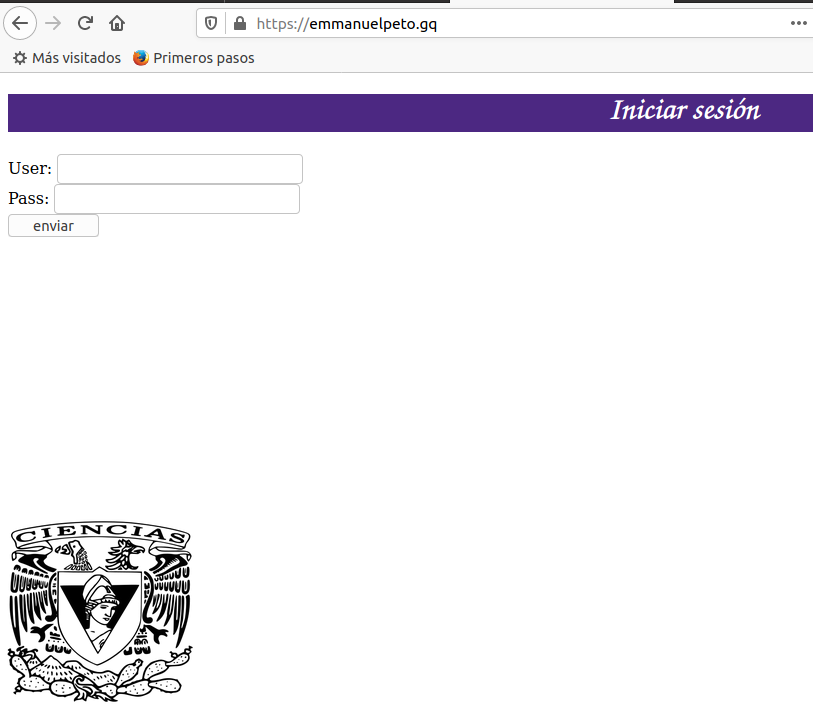
\includegraphics[width=\linewidth]{imagenes/paso10}

Se envió información en el formulario con los valores: usuario $\rightarrow$ \texttt{valentin}, contraseña $\rightarrow$ \texttt{elizalde}.

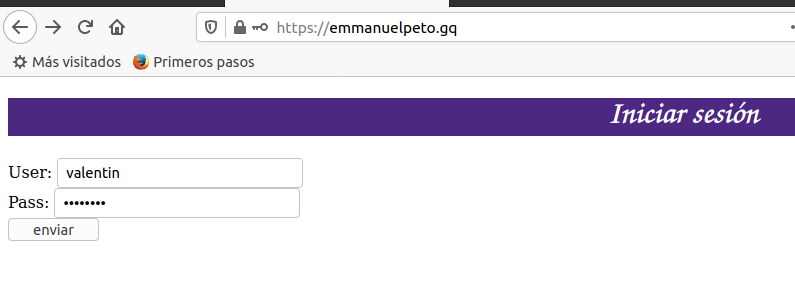
\includegraphics[width=\linewidth]{imagenes/paso11}

Con el método GET se realiza la siguiente captura de tráfico. El protocolo usado para transmitir la información es Transport Layer Security (TLS). Notamos que en la sección \textit{Aplication Data} hay texto cifrado.

\begin{figure}
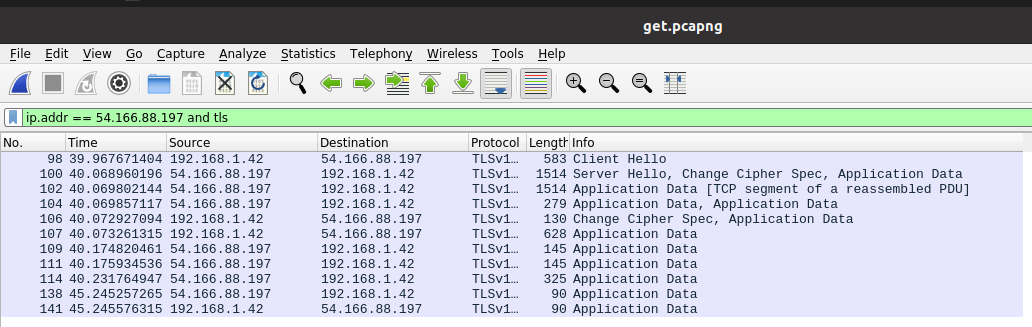
\includegraphics[width=\linewidth]{imagenes/paso12}
\caption{Captura con GET.}
\label{captura1}
\end{figure}

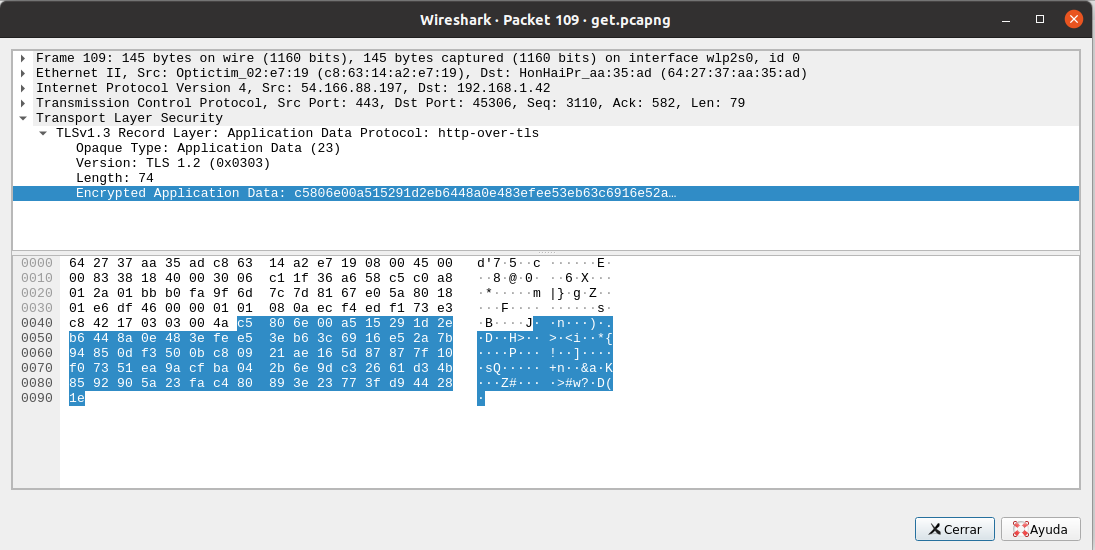
\includegraphics[width=\linewidth]{imagenes/paso13}

La captura con el método POST es similar a la del método GET. También se muestra texto cifrado.

\begin{figure}
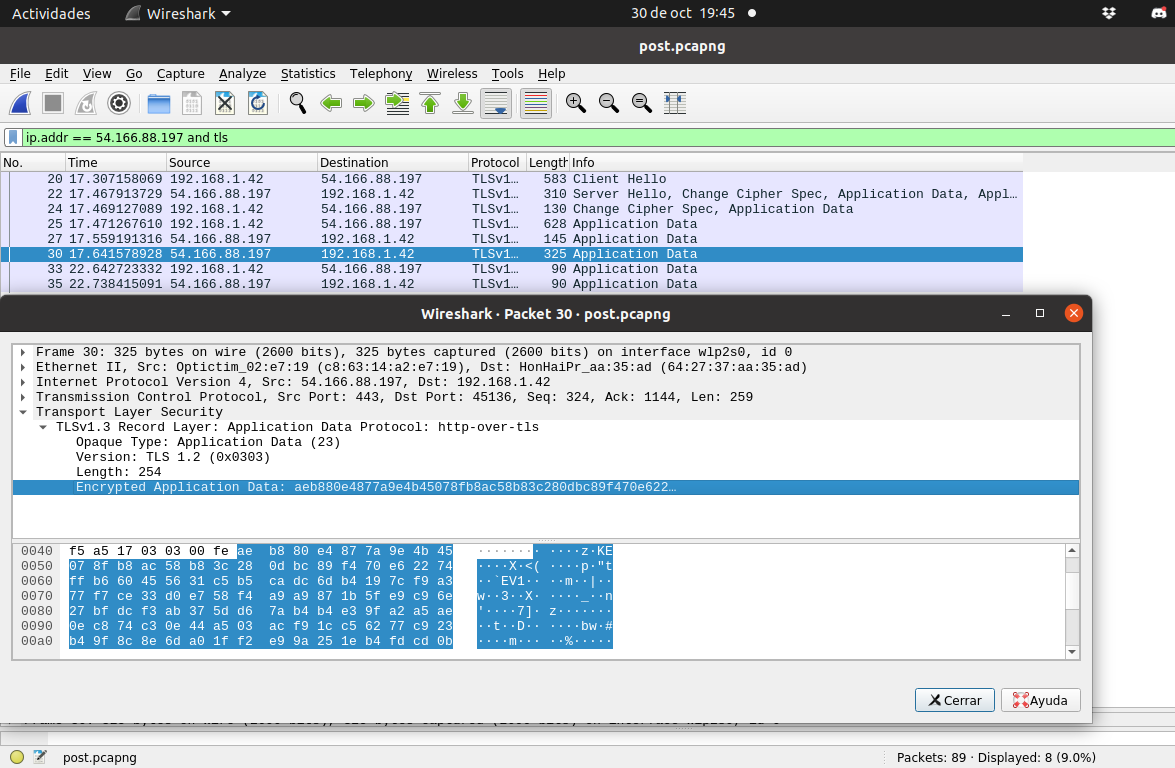
\includegraphics[width=\linewidth]{imagenes/paso14}
\caption{Captura con POST.}
\label{captura2}
\end{figure}

\section{Cuestionario}

\textbf{1. ¿Qué es un DNS?}

Es un sistema distribuido que sirve para traducir un nombre de dominio a una dirección IP.\\

\textbf{2. ¿Qué es un registro A y qué elementos fueron necesarios para registrarlo en el DNS de Freenom?}

Indica que el tipo de registro es de IPv4; es decir, se relaciona un nombre de dominio (\texttt{emmanuelpeto.gq}) con una dirección IPv4 (\texttt{54.166.88.197}).

Para registrarlo en Freenom, primero se verificó que estuviera disponible el nombre del dominio. Después se eligió la terminación \texttt{gq} porque era gratuito. Luego, en la sección \textit{Gestionar dominio}, en la pestaña \textit{Gestionar DNS Freenom} se eligió el tipo A y en \textit{Target} se colocó la IP de la instancia creada en AWS.\\

\textbf{3. ¿Qué es un registro CNAME y Cuál es la diferencia con el registro A?}

Es el nombre canónico de un registro DNS, el cual asigna un alias a un nombre de dominio auténtico.

El registro \texttt{A} guarda la dirección IP de un dominio, mientras que el \texttt{CNAME} guarda un nombre alternativo para el dominio.\\

\textbf{4. ¿Qué es HTTPS? y ¿Por qué es importante para tu seguridad?}

Se utiliza para la transferencia de datos en la capa de aplicación, igual que el protocolo HTTP, pero éste lo hace cifrando los datos.

Es importante porque los usuarios realizamos transferencias bancarias, inicio de sesión, comunicación de datos personales, entre otras cosas, mediante el internet. Si los datos están cifrados no podrán ser interpretados por intrusos en la red hasta que llegen a su destino.\\

\textbf{5. URL creada en la práctica}

\url{https://emmanuelpeto.gq/}\\

\textbf{6. Pantalla de tráfico seguro capturado con wireshark de tu formulario (usar metodo post)}

$\bullet$ Método get: \ref{captura1}

$\bullet$ Método post: \ref{captura2}

\end{document}

